%%%%%%%%%%%%%%%%%%%%%%%%%%%%%%%%%%%%%%%%%
% Journal Article
% LaTeX Template
% Version 2.0 (February 7, 2023)
%
% This template originates from:
% https://www.LaTeXTemplates.com
%
% Author:
% Vel (vel@latextemplates.com)
%
% License:
% CC BY-NC-SA 4.0 (https://creativecommons.org/licenses/by-nc-sa/4.0/)
%
% NOTE: The bibliography needs to be compiled using the biber engine.
%
%%%%%%%%%%%%%%%%%%%%%%%%%%%%%%%%%%%%%%%%%

%----------------------------------------------------------------------------------------
%	PACKAGES AND OTHER DOCUMENT CONFIGURATIONS
%----------------------------------------------------------------------------------------

\documentclass[
	a4paper, % Paper size, use either a4paper or letterpaper
	10pt, % Default font size, can also use 11pt or 12pt, although this is not recommended
	unnumberedsections, % Comment to enable section numbering
	twoside, % Two side traditional mode where headers and footers change between odd and even pages, comment this option to make them fixed
]{LTJournalArticle}

\usepackage{amsmath}

\graphicspath{{Figures/}}

\addbibresource{refs.bib} % BibLaTeX bibliography file

\runninghead{Développez une preuve de concept} % A shortened article title to appear in the running head, leave this command empty for no running head

% \footertext{\textit{Journal of Biological Sampling} (2024) 12:533-684} % Text to appear in the footer, leave this command empty for no footer text

\setcounter{page}{1} % The page number of the first page, set this to a higher number if the article is to be part of an issue or larger work

\newcommand\fref[1]{Figure~\ref{#1}}

%----------------------------------------------------------------------------------------
%	TITLE SECTION
%----------------------------------------------------------------------------------------

\title{Rapport pour le projet : Développez une preuve de concept} % Article title, use manual lines breaks (\\) to beautify the layout

% Authors are listed in a comma-separated list with superscript numbers indicating affiliations
% \thanks{} is used for any text that should be placed in a footnote on the first page, such as the corresponding author's email, journal acceptance dates, a copyright/license notice, keywords, etc
% \author{%
% 	John Smith\textsuperscript{1,2}, Robert Smith\textsuperscript{3} and Jane Smith\textsuperscript{1}\thanks{Corresponding author: \href{mailto:jane@smith.com}{jane@smith.com}\\ \textbf{Received:} October 20, 2023, \textbf{Published:} December 14, 2023}
% }
\author{%
	Thomas Durand-Texte\thanks{Corresponding author: \href{mailto:thomas.durandtexte@protonmail.com}{thomas.durandtexte@protonmail.com}\\ \textbf{Date:} \today}
}


% Affiliations are output in the \date{} command
% \date{\footnotesize\textsuperscript{\textbf{1}}School of Chemistry, The University of Michigan\\ \textsuperscript{\textbf{2}}Physics Department, The University of Wisconsin\\ \textsuperscript{\textbf{3}}Biological Sciences Department, The University of Minnesota}

% Full-width abstract
\renewcommand{\maketitlehookd}{%
	\begin{abstract}
		\noindent
		Ce document vise à présenter le travail réalisé pour le projet "Développez une preuve de concept" de la formation Ingénieur Machine Learning d'OpenClassrooms.
		Le contexte et l'intérêt des méthodes développées dans les articles de la littératures sont présentées et utilisées comme base.
		La méthode "baseline" est la corrélation d'images numérique (communément appelée DIC en anglais).
		Celle-ci est brievement présentée, et est utilisée comme référence afin d'estimer l'apport de la méthode développée.
		Les articles~\cite{Yang:DeepDic2022, WANG:2023107278} présentant les modèles "Deep-DIC" et "DIC-Net" sont utilisées comme base de travail.
		Toutefois, plusieurs modifications sont apportées afin d'améliorer les résultats.
	\end{abstract}
}

%----------------------------------------------------------------------------------------

\begin{document}

\maketitle % Output the title section

%----------------------------------------------------------------------------------------
%	ARTICLE CONTENTS
%----------------------------------------------------------------------------------------

\tableofcontents

\section{A GERER}

A ENONCER : dummy pas valide (on ne retrouverai pas les cartes)
donc faire attention aux validations

\section{Contexte}

Depuis les années 1980, la corrélation d'images numérique (DIC, Digital Image correlation) a connu un fort développement et est actuellement une méthode de mesure de référence pour les mesures de forme et déformations de surface~\cite{Schreir:2010}.
Le principe utilisé est de minimiser la différence entre une image de référence et une image de la surface déformée en estimant de manière itérative une fonction qui permet de passer des coordonnées d'une image à l'autre.
Ce processus peut être effectué sur des sous-images (ou \textit{subsets}, \textit{e.g.} 15~$\times$~15 pixels) avec une fonction polynomiale, ou alors sur l'image (quasi-)complète en estimant le déplacement de points de contrôle d'un maillage.

Bien que largement développé et commercialisé par différentes entreprises, des limitations persistent pour ce groupe de méthodes (il existe de nombreux algorithmes différents):
\begin{enumerate}
	\item le choix de la taille des subsets et de la fonction de forme est délicat à optimiser ;
	\item les effets de bords limitent la précision près des limites de la surface observée ou proche de fissures ;
	\item la précision est limitée pour certains cas, notamment pour l'estimation d'efforts.
\end{enumerate}


Différents travaux de recherche ont étés réalisés ces dernières années pour appliquer les réseaux de neuronnes convolutionnels (CNN) à la corrélation d'images: \cite{Min:2019,Boukhtache:2021,Yang:DeepDic2022,WANG:2023107278, DUAN:2023107234, BOUKHTACHE:2023107367, JIANG:2023103840}.

Les deux articles sur lesquelles le présent travail effectué est basé sont \cite{Yang:DeepDic2022} et \cite{WANG:2023107278}.
Les deux modèles utilisent une architecture de type de U-Net \cite{ronneberger:2015}.
Pour "Deep-DIC", le dataset est composée d'images synthétiques et les données cibles, \textit{i.e.} déplacement et déformation, correspondent à un mouvement de coprs rigide et un gaussienne.
Pour "DIC-Net", le dataset est partiellement composé d'images réelles, et les déformées sont calculées avec des éléments finis de Hermite.
Dans les deux cas, les images initiales sont utilisées pour générer des paires d'images, une image de référence et une image déformée, à partir des déformations (aléatoires) cibles.
De plus, pour limiter la redondances des informations locales, les images rognées aléatoirement pour obtenir une paire d'images de taille 128~$\times$~128.


\textbf{VOIR ANNONCE PLAN}
Le dataset et les images originales de l'article \cite{WANG:2023107278} étant basé de Baidu Netdisk, le choix ici est de générer un dataset à partir d'images numériques, à l'instar de Yang \textit{et al.}~\cite{Yang:DeepDic2022} en utilsant le protocle de Wang \textit{et al.}~\cite{WANG:2023107278}, à savoir la génération d'images déformée avec des éléments de Hermite.

Des codes sont disponibles sur \url{https://github.com/YinWang20/DIC-Net} et sont utilisés comme base, mais des modifications ont été effectuées.
Notamment, pour la génération des images déformées, les codes proposées sont en Matlab\textregistered{} et ont donc dû être implémentés en Python.


\section{Génération du dataset}

Le dataset est composé de pairs d'images : une image de référence et une image dite déformée.
L'objectif du modèle est d'estimer le déplacement de chaque pixel entre l'image de référence et l'image déformée, ainsi que les dérivées spatiales du déplacement.

Afin de générer une pair d'image, il faut une première image d'un mouchetis.
Cette étape étant gourmande en ressources, cette première image va être utilisée pour générer, sur le tas, 16 nouvelles images.
Puis, chaque image va être interpolée pour créer une paire d'image.
Afin de diminuer les temps de calcul requis, l'implémentation du dataset est réalisée avec deux pairs de dataset / dataloader :

\begin{enumerate}
	\item génération et stockage des images initiales (RAM)
	\item transformation des images initiales (sur le tas) et calcul de la pair d'image
\end{enumerate}

Toutes les opérations sont réalisées dans la mémoire vive, donc aucune image n'est enregistrée.
De plus, contrairement aux méthodes précédentes, les réseaux de neuronnes voeint toujours de nouvelles images.

\subsection{protocole pour une pair d'images}
Le protocole de génération d'une pair d'image est affiché \fref{fig:ds_protocol}.

\begin{figure}[!ht]
	\begin{center}
		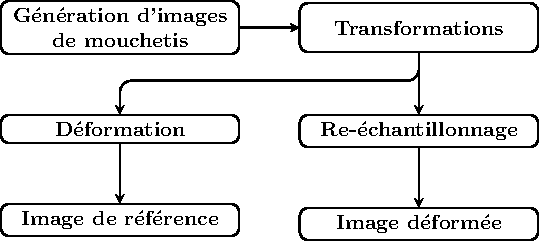
\includegraphics[width=80mm]{dataset/protocol.pdf}
	\end{center}
	\caption{Protocole pour générer une pair d'image}
	\label{fig:ds_protocol}
\end{figure}

Chaque image initiale est transformée afin de générer plus images.
Les 3 transformations suivantes sont appliquées:
\begin{itemize}
	\item négatif de l'image ($\times$2)
	\item miroir horizontal ($\times$2)
	\item rotation de l'image de 90° ($\times$4)
\end{itemize}
En combinant les transformations, au total 16 images sont générées à partir d'une première image.

\subsection{Génération d'images de mouchetis}

\subsection{Image de référence}
Afin de simplifier la mise en équation du problème, l'image de référence est calculée en interpolant l'image avec l'algorithme suivant:
\begin{enumerate}
	\item choix aléatoire d'une taille de maillage ;
	\item génération aléatoire des déplacements et déformations ;
	\item calcul des positions dans l'image initiale de chaque pixel ($u^{def}, v^{def}$) = ($u^{ref}+\Delta u$, $v^{ref}+\Delta v$) ;
	\item interpolation de l'image initiale aux positions ($u^{def}, v^{def}$).
\end{enumerate}
À noter que, ici, les positions ($u^{ref}, v^{ref}$) correspondent à un maille de 128~$\times$~128 pixels (0 $\rightarrow$ 127, 0 $\rightarrow$ 127), et que le déplacement ($\Delta u, \Delta v$) et les déformations ($\partial \Delta u / \partial u$, $\partial \Delta u / \partial v$, $\partial \Delta v / \partial u$, $\partial \Delta v / \partial v$) sont calculés à l'aide d'un maillage d'élements finis de Hermite (voir \cite{WANG:2023107278} pour les détails de calculs).


\subsection{Image déformée}
Pour obtenir l'image dite déformée, un simple ré-échantillonnage est réalisé en fonction des positions ($u^{def}, v^{def}$), et ce afin que la totalitée de l'information de l'image de référence soit contenue dans l'image déformée.
Les étapes de calcul sont :
\begin{enumerate}
	\item calcul des valeurs minimales et maximales de $u^{def}$ et $v^{def}$, floor et ceil $\rightarrow$ ($u_0, u_1, v_0, v_1$)
	\item génération d'un maillage de 128$~\times$~128~pixels ($u_0 \rightarrow u_1$, $v_0 \rightarrow v_1$)
	\item interpolation de l'image initiale aux points du maillage
\end{enumerate}
avec ($u_0, u_1$) encadrant (min($u^{def}$), max($u^{def}$)), et ($v_0, v_1$) encadrant (min($v^{def}$), max($v^{def}$)).

Cette opération de ré-échantillonnage va cependant modifier les valeurs de déplacement et déformations.
Il est donc nécessaire de recalculer les valeurs correspondantes dans le repère de l'image initiale.

Pour une position ($u^{rs}, v^{rs}$) dans le repère de l'image ré-echantillonnée, la position correspondante dans le repère initial est ($u_0 + u^{rs}*\alpha_u$, $v_0 + v^{rs}*\alpha_v$), avec $\alpha_u = u_1 - u_0$ et $\alpha_v = v_1 - v_0$.
Donc pour passer du repère initial au repère ré-échantillonné, on a :
\begin{equation}
	\left(
		\begin{array}{l}
			u^{rs} \\
			v^{rs} \\
		\end{array}
	\right)
	=
	\left(
		\begin{array}{l}
			(u^{ref} + \Delta u - u_0) / \alpha_u\\
			(v^{ref} + \Delta v - v_0) / \alpha_v
		\end{array}
	\right) \quad .
\end{equation}
Les valeurs de déplacement et déformées dans le repère ré-échantillonné par rapport aux positions ($u^{ref}$, $v^{ref}$) sont obtenus avec :
\begin{equation}
	\left(
		\begin{array}{c}
			\Delta u^{rs}\\
			\Delta v^{rs}\\
			\epsilon_{xx}^{rs}\\
			\epsilon_{xy}^{rs}\\
			\epsilon_{yx}^{rs}\\
			\epsilon_{yy}^{rs}
		\end{array}
	\right)
	=
	\left(
		\begin{array}{c}
			u^{rs} - u^{ref}\\
			v^{rs} - v^{ref}\\
			\partial \Delta u^{rs} / \partial u^{ref}\\
			\partial \Delta u^{rs} / \partial v^{ref}\\
			\partial \Delta v^{rs} / \partial u^{ref}\\
			\partial \Delta v^{rs} / \partial v^{ref}\\
		\end{array}
	\right)
\end{equation}

\begin{equation}
	\left(
		\begin{array}{c}
			\Delta u^{rs}\\
			\Delta v^{rs}\\
			\epsilon_{xx}^{rs}\\
			\epsilon_{xy}^{rs}\\
			\epsilon_{yx}^{rs}\\
			\epsilon_{yy}^{rs}
		\end{array}
	\right)
	=
	\left(
		\begin{array}{c}
			(u^{ref} (1 - \alpha_u) + (\Delta u -u_0)) / \alpha_u\\
			(v^{ref} (1 - \alpha_v) + (\Delta v -v_0)) / \alpha_v\\*
			((1 - \alpha_u) + (\partial \Delta u / \partial u^{ref})) / \alpha_u\\
			(\partial \Delta u / \partial v^{ref}) / \alpha_u\\
			(\partial \Delta v / \partial u^{ref}) / \alpha_v\\
			((1 - \alpha_v) + (\partial \Delta v / \partial v^{ref})) / \alpha_v
		\end{array}
	\right)
\end{equation}

Ainsi, pour obtenir les valeurs recherchées :
\begin{equation}
	\left(
		\begin{array}{c}
			\Delta u\\
			\Delta v\\
			\epsilon_{xx}\\
			\epsilon_{xy}\\
			\epsilon_{yx}\\
			\epsilon_{yy}
		\end{array}
	\right)
	=
	\left(
		\begin{array}{c}
			u^{def} - u^{ref}\\
			v^{def} - v^{ref}\\
			\partial \Delta u / \partial u^{ref}\\
			\partial \Delta u / \partial v^{ref}\\
			\partial \Delta v / \partial u^{ref}\\
			\partial \Delta v / \partial v^{ref}\\
		\end{array}
	\right) \quad ,
\end{equation}
il faut alors utiliser :
\begin{equation}
	\left(
		\begin{array}{c}
			\Delta u\\
			\Delta v\\
			\epsilon_{xx}\\
			\epsilon_{xy}\\
			\epsilon_{yx}\\
			\epsilon_{yy}
		\end{array}
	\right)
	=
	\left(
		\begin{array}{c}
			\alpha_u \Delta u^{rs} - u^{ref} * (1 - \alpha_u) + u_0\\
			\alpha_v \Delta v^{rs} - v^{ref} * (1 - \alpha_v) + v_0\\
			\alpha_u \epsilon_{xx}^{rs} - (1-\alpha_u)\\
			\alpha_u \epsilon_{xy}^{rs}\\
			\alpha_v \epsilon_{yx}^{rs}\\
			\alpha_v \epsilon_{yy}^{rs} - (1-\alpha_v)\\
		\end{array}
	\right) \quad .
\end{equation}

Le modèle réalisé intègre directement cette transformation.
Il prend donc en entrée :
\begin{itemize}
	\item la pair d'images ;
	\item les positions ($u^{ref}$, $v^{ref}$) ;
	\item les informations de ré-échantillonnage ($u_0$, $v_0$, $\alpha_u$, $\alpha_v$).
\end{itemize}

\section{Corrélation d'images numériques}
La corrélation d'image numérique est une méthode largement utilisée depuis plus de 40~ans.
Il s'agit d'une des mesures de références pour la recherche et l'industrie~\cite{Schreir:2010}.
Les de la méthode de base sont assez simple à comprendre, et, si l'on ignore les distortion optiques, sa mise en oeuvre est relativement simple et rapide.

À noter que, ici, pour simplifier les algorithmes, les variations d'illumination ne sont pas prises en comptes puisque les images sont normalisées et que les variations locales d'illumination ne sont pas simulées.
Une amélioriation possible du dataset est donc de simuler des variations locales d'illumination.

Le principe pour un cas 1D est présenté sur la \fref{fig:dic_1d}.
À partir du gradient de l'image de référence ($\partial F(x) / \partial x$) et de la différence entre les deux images ($\Delta I = G(x)-F(x)$), le décalage $\Delta x$ est retrouvé avec~:
\begin{equation}
	\Delta x = - \dfrac{\Delta I}{\partial F(x) / \partial x}
\end{equation}

\begin{figure}[!ht]
	\begin{center}
		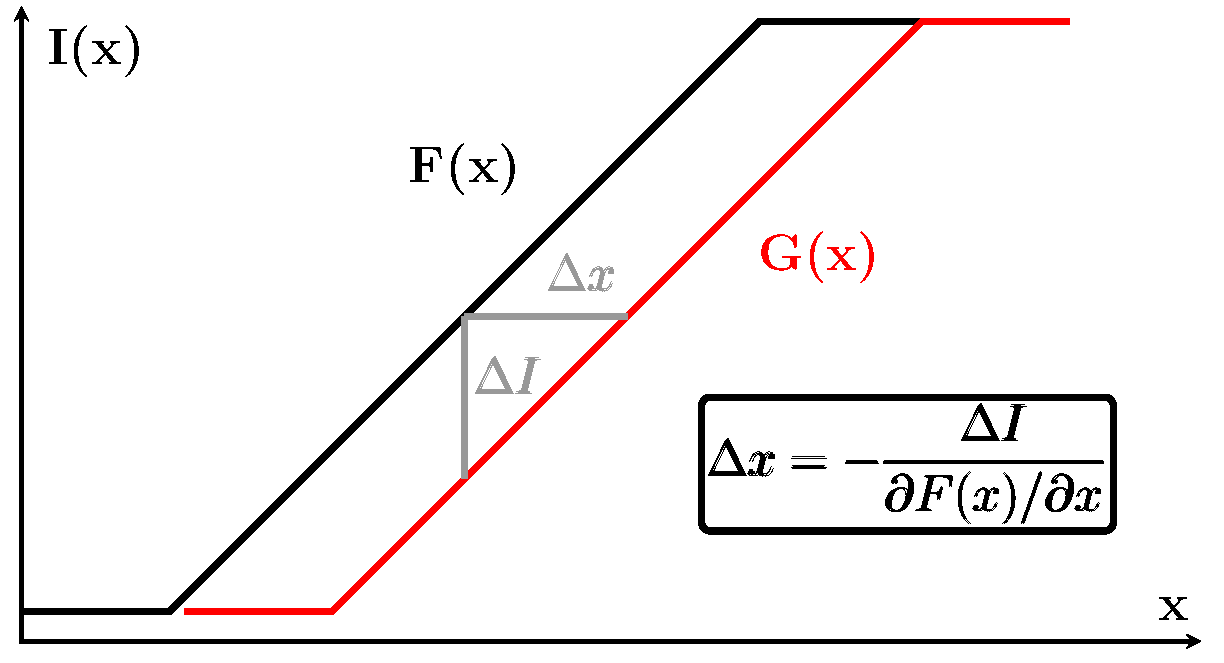
\includegraphics[width=70mm]{dic/cas1d.pdf}
	\end{center}
	\caption{Principe de la corrélation d'image pour le cas 1D}
	\label{fig:dic_1d}
\end{figure}

Lorsque l'on traite des images, l'estimation de $\Delta x$ est effectué sur une surface, avec une approximation (le plus souvent) polynomiale d'ordre 2~: $\Delta x(u, v) = p_0 + p_1u + p_2v + p_3u^2 + p_4 uv + p_5 v^2$.
Deux polynomes sont alors utilisés, $p_u$ pour $\Delta u$ et $p_v$ pur $\Delta v$.

Les deux polynomes sont estimé de manière itératif à l'aide d'une estimation par moindre carré.
En définissant une base de fonction $\phi_i(u, v)$, ($1$, $u$, $v$, $u^2$, etc...), l'estimateur est construit tel que:

\begin{equation}
	M = [A^T A]^{-1} A^T
\end{equation}
avec
\begin{equation}
	A = \left[
		\begin{array}{c}
			\Phi(u, v) * F_u(u, v)
			\\ \hline
			\Phi(u, v) * F_v(u, v)
		\end{array}
	\right] \quad ,
\end{equation}
$\Phi(u, v)$ étant une matrice à 6 lignes ($\phi_0(u, v)$, $\phi_1(u, v)$, ...), $F_u(u, v)$ et $F_v(u, v)$ étant les dérivées spatialles de $F(u, v)$ selon les axes $u$ et $v$ respectivement.
À noter que chaque ligne de $\Phi(u, v)$ est multipliée par $F_{u/v}(u,v)$, $\Phi(u, v) * F_u(u,v)$ n'est donc pas une opération matricielle.

En partant d'une position suffisamment proche de la solution, les polynomes $p_u$ et $p_v$ sont obtenus avec~:
\begin{equation}
	\left(
	\begin{array}{c}
		\Delta p_u\\
		\Delta p_v
	\end{array}
	\right)
	=
	M (F(u,v) - G(u,v)) \quad .
\end{equation} 
Avec un approche itératif, $p_u$ et $p_v$ sont estimé avec l'algorithme~:
\begin{enumerate}
	\item calculer ($u_{def}, v_{def}$) = f($p_u, p_v, u, v$)~;
	\item interpoler $G(u_{def}, v_{def})$~;
	\item estimer $\Delta p_u$ et $\Delta p_v$~;
	\item estimer $p_u^{i}$ et $p_v^{i}$ par moindres carrés tel que f($p_u^{i}, p_v^{i}, u, v)$ $\approx$ f($p_u^{i-1}, p_v^{i-1}$,f($\Delta p_u, \Delta p_v, u, v)$) 
\end{enumerate}

Un example d'estimation est affiché sur la \fref{fig:dic_example}.
La déformation estimée est visiblement d'ordre 2.

\begin{figure}[!ht]
	\begin{center}
		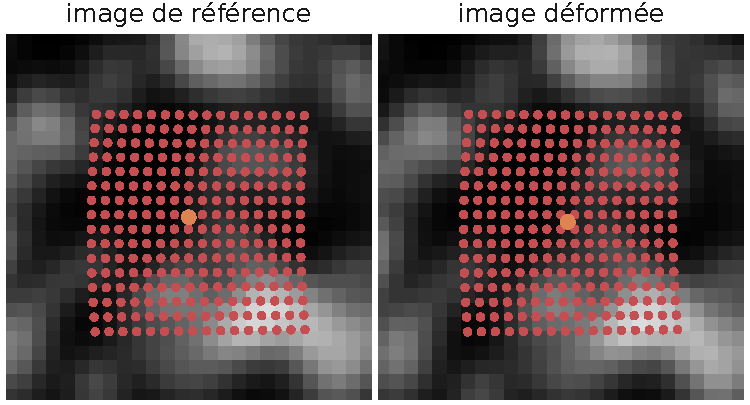
\includegraphics[width=80mm]{dic_example.pdf}
	\end{center}
	\caption{Example d'estimation de déformation, les points rouges correspondent aux positions des pixels dans l'image de référence (initialisation à gauche) et dans l'image déformée (estimation à droite).}
	\label{fig:dic_example}
\end{figure}


\section{Modèle Deep Learning}

\subsection{Architecture}

\subsection{Modifications}

\subsection{Entrainement simultané}

%----------------------------------------------------------------------------------------
%	 REFERENCES
%----------------------------------------------------------------------------------------

\printbibliography % Output the bibliography

%----------------------------------------------------------------------------------------

\end{document}
